\modeCorrection


\renewcommand{\thesubsection}{\textcolor{red}{\Roman{section}.\arabic{subsection}}}
\renewcommand{\thesubsubsection}{\textcolor{red}{\Roman{section}.\arabic{subsection}.\alph{subsubsection}}}
\renewcommand{\titreDocu}[1]{
  \refstepcounter{document} % update counter
  \textbf{Exercice \arabic{document} -- #1} 
  \addcontentsline{toc}{document}{\protect\numberline{} #1} % update table of content
}

\setcounter{section}{0}
\setcounter{document}{0}


\nomPrenomClasse
\vspace{1cm}

\begin{center}
\begin{mdframed}[style=titr, leftmargin=60pt, rightmargin=60pt, innertopmargin=7pt, innerbottommargin=7pt, innerrightmargin=8pt, innerleftmargin=8pt]
\begin{center}
\begin{Large}
    Devoir Surveillé n°2 : Solutions aqueuses (30min)
\end{Large}
\end{center}
\end{mdframed}
\end{center}
\vspace{1cm}

\begin{tableauCompetences}
    APP & S'approprier les informations d'un document & & & & \\
    \hline
    REA & Utiliser une grandeur quotient 
pour déterminer le numérateur ou le dénominateur  & & & & \\
\hline
    ANA &  Exploiter les informations extraites des données & & & & 
\end{tableauCompetences}

\begin{tcolorbox}[colback=red!5!white,colframe=red!75!black,title=\textbf{Consignes : }]
   \begin{enumerate}
        \item Vous rédigez tout sur le sujet,
        \item N'oubliez pas les unités dans vos résultats, 
        \item La calculatrice \underline{n'est pas autorisée}.
   \end{enumerate}
\end{tcolorbox}

\begin{doc}{Quizz \begin{large}
    /6,5 points
\end{large}}
Entourer \underline{la ou les} bonne(s) réponse(s) :
\begin{enumerate}
    \item \textbf{Le sang est un liquide dont l'eau est : (1pt)}
        \begin{align*}
            %a.& ~\text{le soluté} & b.& ~\text{ le solvant} & c.& ~\text{la solution}
            a.& ~\text{le soluté} & b.& ~\text{ \textcolor{red}{le solvant}} & c.& ~\text{la solution}
        \end{align*}
    \item \textbf{Un échantillon de 10 g d’aspirine est dissous dans 50 cL d’eau. La concentration
en masse d’aspirine dans la solution acqueuse est : (1pt)}
        \begin{align*}
            %a.& \text{ 20 g.L$^{-1}$} & b.& \text{ 0,2 g.L$^{-1}$} & c.& ~\text{ 200 g.L$^{-1}$}
            a.& \text{ \textcolor{red}{20 g.L$^{-1}$}} & b.& \text{ 0,2 g.L$^{-1}$} & c.& ~\text{ 200 g.L$^{-1}$}
        \end{align*}
    \item \textbf{On place un cachet de 1000 mg d'aspirine dans un verre contenant un volume de 25 cL d'eau. On agite avec une cuillère. On a réalisé : (1,5pts) }
        \begin{align*}
            %a.& ~\text{Une dilution} & b.& ~\text{Une dissolution} & c.& ~\text{Une solution fille} & d.& ~\text{Une solution aqueuse}
            a.& ~\text{Une dilution} & b.& ~\text{\textcolor{red}{Une dissolution (1pt)} } & c.& ~\text{Une solution fille} & d.& ~\text{\textcolor{red}{Une solution aqueuse (0.5pt)}} 
        \end{align*}
    \item \textbf{La concentration en masse d'aspirine de la solution obtenue à la question précédente est : (1pt)}
        \begin{align*}
            %a.& ~\text{ 25 g.L$^{-1}$} & b.& ~\text{ 40 mg.L$^{-1}$} & c.& ~\text{4 g.L$^{-1}$}
            a.& ~\text{25 g.L$^{-1}$} & b.& ~\text{40 mg.L$^{-1}$} & c.& ~\text{\textcolor{red}{4 g.L$^{-1}$}}
        \end{align*}
    \item \textbf{On rajoute 25 cL d'eau dans le verre : (2pts)}
        %\begin{enumerate}[label=\textit{\alph*.}, align=left, leftmargin=*]
        %    \item la solution obtenue est moins concentrée en aspirine
        %    \item la masse d'aspire dans le verre est 2000 mg 
        %    \item la concentration en masse d'aspirine est deux fois plus grande 
        %    \item la concentration en masse d'aspirine vaut 2g.L$^{-1}$
        %\end{enumerate}
        \begin{enumerate}[label=\textit{\alph*.}, align=left, leftmargin=*]
            \item \textcolor{red}{La solution obtenue est moins concentrée en aspirine}
            \item la masse d'aspire dans le verre est 2000 mg
            \item la concentration en masse d'aspirine est deux fois plus grande 
            \item \textcolor{red}{la concentration en masse d'aspirine vaut 2g.L$^{-1}$}
        \end{enumerate}
\end{enumerate}
\end{doc}

\begin{doc}{Retour sur le colorant bleu E131 \begin{Large}
    /8,5 points
\end{Large}}
\begin{wrapfigure}{r}{0.2\textwidth}
\vspace{-1cm}
    \centering
      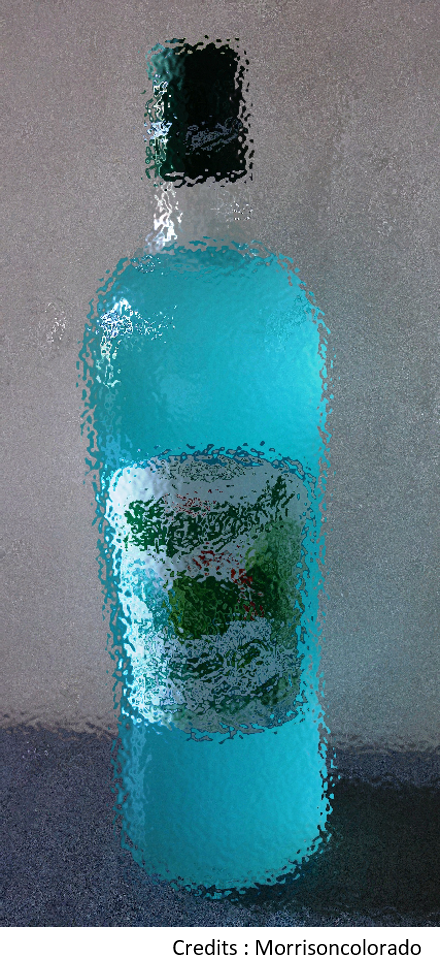
\includegraphics[scale=0.35]{Images/DS/DS2/Sirop_menthe.png}
  \end{wrapfigure}
Certains sirops de menthe de couleur bleue utilise un colorant alimentaire appelé E131. \textbf{On cherche à déterminer la concentration en masse de ce colorant}, qu'on notera $C_{m,com}$, d'un sirop de menthe commercial à l'aide d'un dosage.\\
Pour cela, on réalise \textbf{une échelle de teintes} constituées de quatre solutions fille étalons notées S$_1$, S$_2$, S$_3$ et S$_4$, de volume $V_{f}=20,0$~mL, obtenues après dilution d'une solution mère de concentration en masse de colorant E131 $C_{m,m}=12,0$~mg.L$^{-1}$. On note $V_{m}$ le volume de solution mère prélevé pour obtenir les solutions filles.\\
\begin{tabular}{|C{0.6}|C{0.13}|C{0.13}|C{0.13}|C{0.13}|}
    \hline
    \cellcolor{orange!25} Solution fille & S$_1$ & S$_2$ & S$_3$ & S$_4$ \\
    \hline
    \cellcolor{orange!25} V$_m$ (en mL) & 13,3 & 10,0 &  & 2,5 \\
    \hline 
    \cellcolor{orange!25} V$_f$ (en mL) & 20,0 & 20,0 & 20,0 & 20,0 \\
    \hline
    \cellcolor{orange!25} Facteur de dilution F & 1,5 & 2,0 & & 8,0 \\
    \hline
    \cellcolor{orange!25} Concentration en masse solution fille $C_{m,f}$ (en mg.L$^{-1}$) & 8,0 & 6,0 & 3,0 & 1,5 \\
    \hline
\end{tabular}
\\

\question{En détaillant les calculs, compléter le tableau de l'énoncé. (3pts) }{
\begin{equation*}
    F = \frac{C_{m,m}}{C_{m,f}} ~(1pt)~= \frac{12,0}{3,0} = 4,0 ~(0,5+0,5=1pt)
\end{equation*}
On en déduit le volume $V_m$ :
\begin{equation*}
    V_m = \frac{V_f}{F}~(1pt) = \frac{20,0}{4,0} = 5,0~(0,5+0,5=1pt)
\end{equation*}
Voici le tableau complété (0,5pt):\\
\begin{tabular}{|C{0.35}|C{0.13}|C{0.13}|C{0.13}|C{0.13}|}
    \hline
    \cellcolor{orange!25} Solution fille & S$_1$ & S$_2$ & S$_3$ & S$_4$ \\
    \hline
    \cellcolor{orange!25} V$_m$ (en mL) & 13,3 & 10,0 & \textcolor{red}{5,0} & 2,5 \\
    \hline 
    \cellcolor{orange!25} V$_f$ (en mL) & 20,0 & 20,0 & 20,0 & 20,0 \\
    \hline
    \cellcolor{orange!25} Facteur de dilution F & 1,5 & 2,0 & \textcolor{red}{4,0} & 8,0 \\
    \hline
    \cellcolor{orange!25} Concentration en masse solution fille $C_{m,f}$ (en mg.L$^{-1}$) & 8,0 & 6,0 & 3,0 & 1,5 \\
    \hline
\end{tabular}}{0}
\\
\vspace{-5pt}
\question{Le sirop de menthe est dilué 10 fois. La teinte du sirop de menthe dilué est comprise entre celle des solutions S$_1$ et S$_2$. Déterminer un encadrement de la concentration en masse de la solution de menthe dilué. (1pt)}{\begin{equation*}
    6,0~\text{mg.L$^{-1}$} < C_{m,\text{sirop dilué} }< 8,0~\text{mg.L$^{-1}$}
\end{equation*}}{0}
\\
\vspace{-5pt}
\question{En déduire un encadrement de $C_{m,com}$. (1pt)}{Comme on a dilué 10 fois, les valeurs de l'encadrement précédent doivent être multipliées par 10 ce qui donne :
\begin{equation*}
    60~\text{mg.L$^{-1}$} < C_{m,com} < 80~\text{mg.L$^{-1}$}
\end{equation*}}{0}
\\
\vspace{-5pt}
\question{Choisir la verrerie pour diluer le sirop de menthe. \textbf{Vous ferez attention à donner des valeurs correctes des volumes de chaque verrerie utilisée.} (2,5pts)}{Verrerie pour une dilution par 10 de la solution mère : un bécher pour contenir le sirop (0,5pt), une pipette jaugée de 10,0 mL pour prélever le sirop dans le bécher (0,5+0,5=1pt), une
fiole jaugée de 100,0 mL pour avoir un facteur de dilution de 10 ($V_{\text{fiole}}=10\times V_{\text{prélevé}}$) (0,5+0,5=1pt)}{0}
\\
\vspace{-5pt}
\question{Proposer une méthode pour diminuer l'incertitude sur la concentration en masse de la solution commerciale (1pt).}{On pourrait réaliser plus de solutions filles dont les concentrations seraient comprises entre 6,0 mg.L$^{-1}$ et 8,0 mg.L$^{-1}$.\\
On peut également réaliser une courbe d'étalonnage en mesurant la masse volumique de solutions contenant du colorant E131 en fonction de leur concentration en masse de ce colorant puis mesurer la masse volumique du sirop (préalablement dilué) et en déduire sa concentration en masse par lecture graphique.}{0}
\end{doc}

%\begin{center}
 %   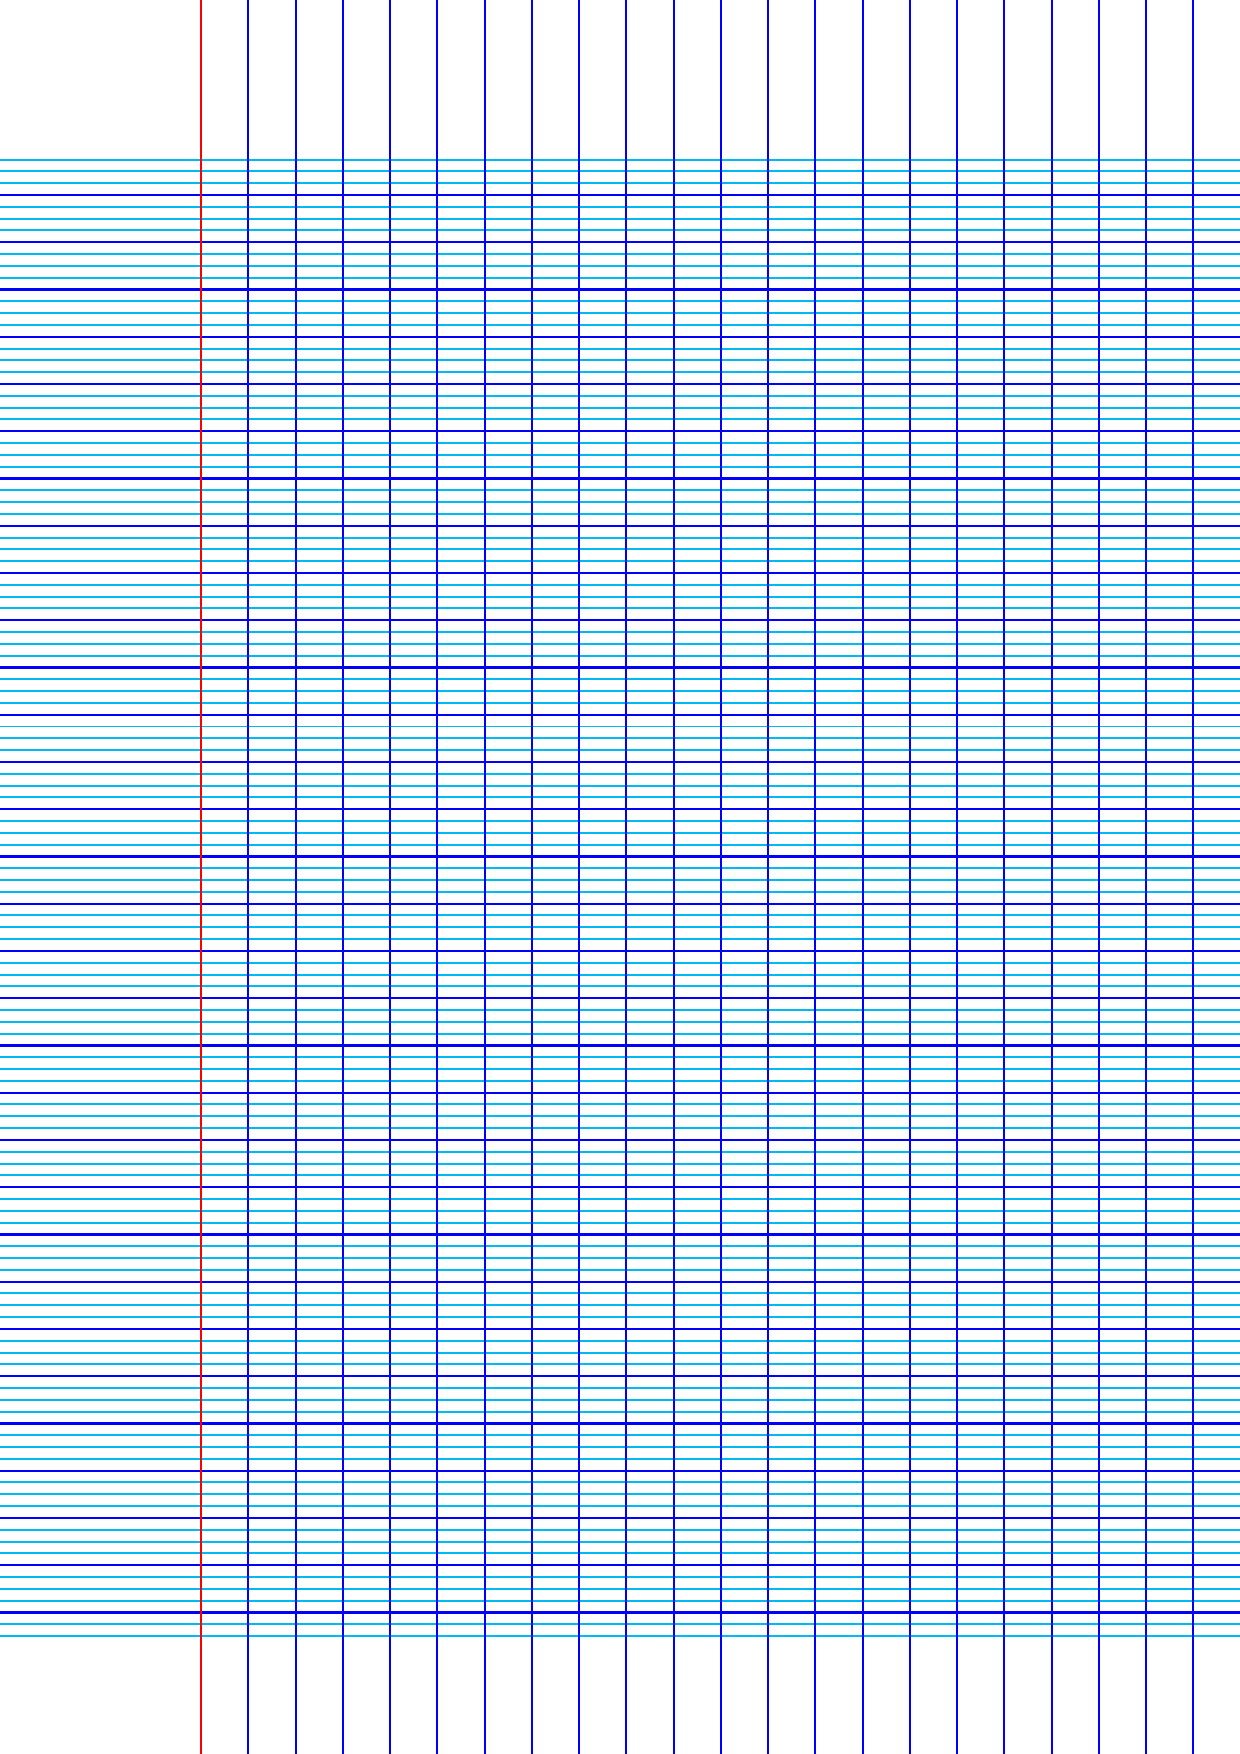
\includegraphics[scale=0.85]{Images/Feuilles/Grands_carreaux.pdf}
%\end{center}